\begin{savequote}[75mm]
What I cannot create, I do not understand.
\qauthor{Richard Feynman}
\end{savequote}

% pending plagiarism check
\begin{flushleft}
\chapter{Image-based profiling to identify revertant therapeutics in pre-malignant models of colon cancer}

\section{Motivation}

Based on the observation that (1) joint representations of organoid morphology and biochemical state can be learned, and (2) small molecule perturbations can shift organoids in representation space, the following hypothesis can be formulated: If well-annotated small molecules can help identify a causal representation of unknown organoid states, unknown small molecules with desirable properties can be identified by their ability to shift the state of well-annotated organoid models. 
Put differently, instead of using small-molecule perturbations to learn about the biology of non-characterized patient derived organoids, we should be able to use genetically engineered organoid models to learn about desirable properties of non-characterized small molecules.

The emergence of colorectal cancer via the chromosomal instability process is a well understood sequence of genetic events that start with hyperactivation of canonical Wnt signaling, often via loss of APC, followed by the hyperactivation of RAS-MAPK signaling, often via oncogenic mutations of KRAS. These two mutations are frequent and signficantly co-occuring in colorectal cancer patients, suggesting an interplay between these two acquired genetic functional events that lead to a selfish evolutionary advantage of premalignant cells. While the genetic events within this process are well understood, no therapeutics targeting the loss of APC or the hyperactivation of KRAS via the frequent G12D activation have yet been developed. 

\begin{figure}[h]
\centering
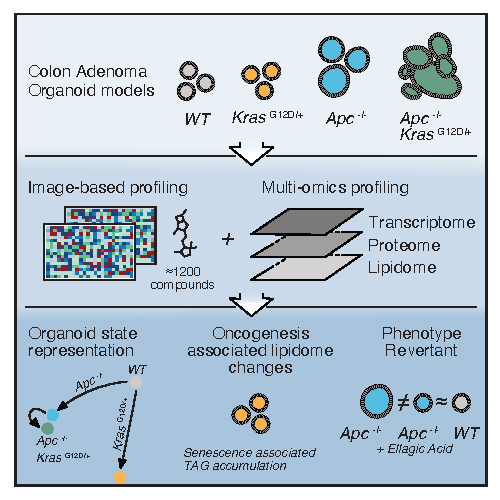
\includegraphics[width=250,
                height=\textheight,
                keepaspectratio]{figures/adenomaprofiling/pdf/fig_0_2.pdf}
\caption{\textbf{Visual abstract of adenoma model profiling project.}}
\label{fig_a02}
\end{figure}
\bigbreak


By using image-based profiling of genetically engineered mouse colon organoid models carrying Apc truncating mutations and/or a Kras G12D allele, I modelled the first set of genetic events within the Adenoma-Carcinoma sequence. Using a similar strategy than in the first chapter of this thesis, organoid models were characterized in-depth and subjected to a high-throughput small molecule screen of ca. 1700 FDA-approved substances and experimental compounds. The goal of this project was to (1) understand the biological state changes caused by individual transforming genetic changes in Apc and Kras within colon epithelial cells and (2) identify putative candidates that shift organoid states within the learned representation away from a pre-malignant state. 


\begin{figure}[H]
\centering
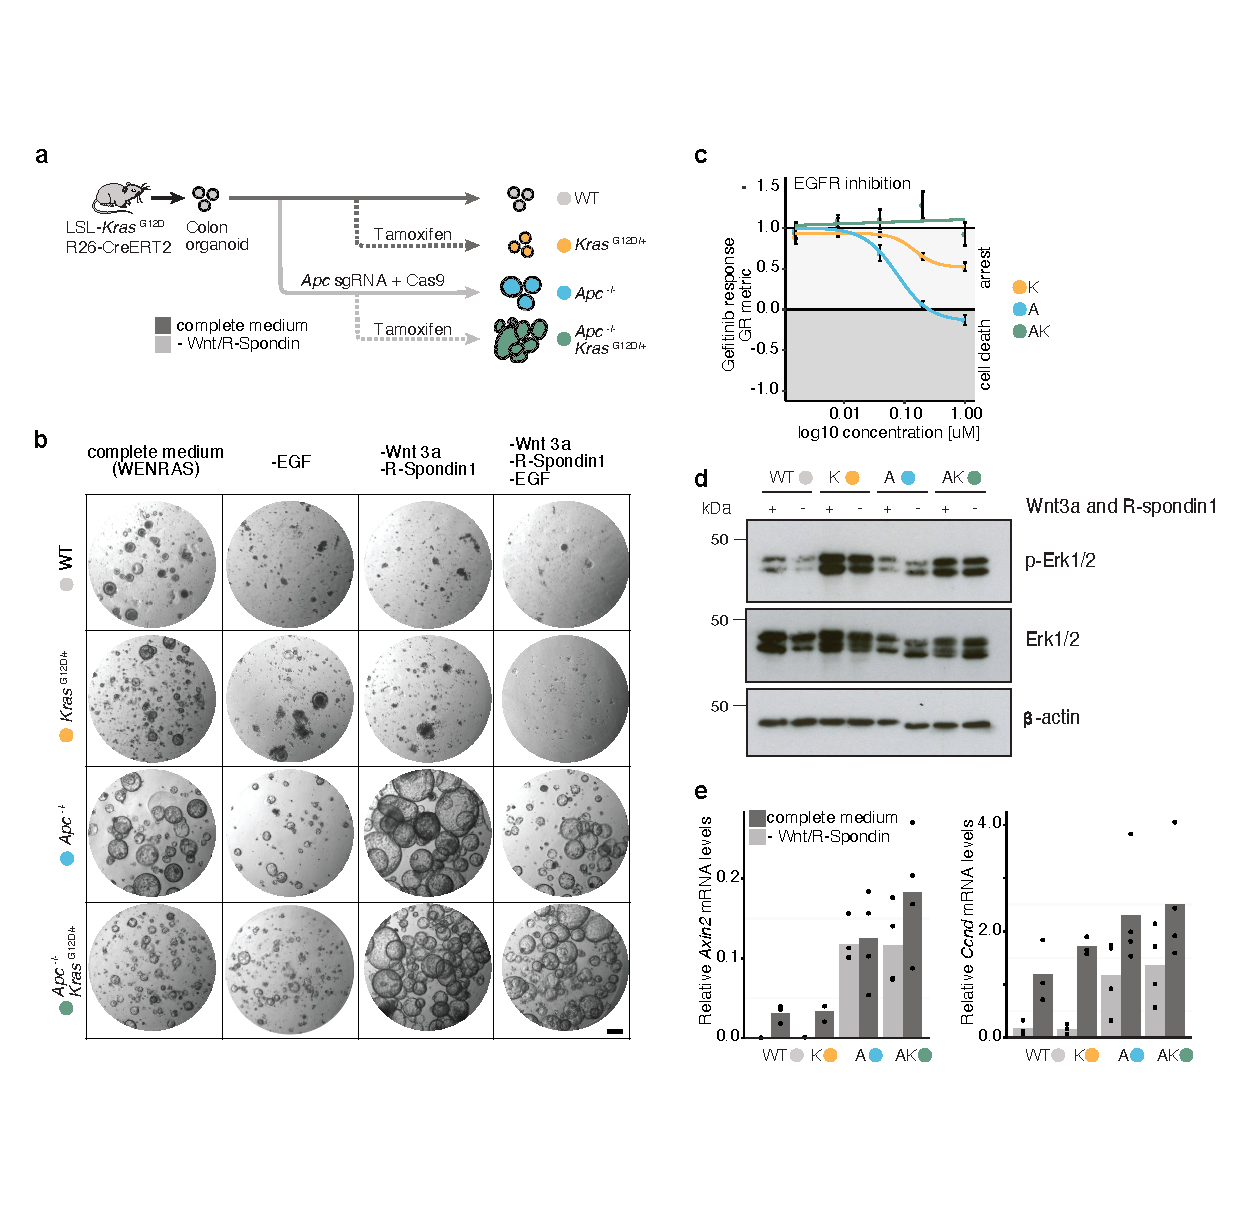
\includegraphics[width=\textwidth,
                height=\textheight,
                keepaspectratio]{figures/adenomaprofiling/pdf/fig_1_0.pdf}
\caption{\textbf{Establishing organoid models of colon adenoma, a} Overview of organoid model establishment. Mouse colon organoids were isolated from a transgenic donor animal carrying an inactive conditional oncogenic KrasG12D allele. Homozygous truncation of Apc via CRISPR and activation of the heterozygous KrasG12D allele lead to four different genetically defined organoid models.
\textbf{b} In vitro growth factor dependency of adenoma models. Organoids were cultured in complete or modified medium containing combinations of Wnt3A, R-Spondin1-Fc and EGF for 120h and subsequently imaged. Scalebar = 200um.
\textbf{c}	Oncogenic KrasG12D increases resistance to Egfr inhibition. Organoid ATP levels were measured 4 days after Gefitinib treatment and adjusted for organoid growth rate. Points represent mean of n=2 independent experiments. Error bars represent standard error of mean.  
\textbf{d} Erk phosphorylation is increased by oncogenic KrasG12D. Organoid models were cultured with or without Wnt3A and R-Spondin1-Fc for 72h and analyzed for protein levels. p, phospho.   
\textbf{e}	Loss of Apc induces transcription of canonical Wnt-signaling target genes. qRT–PCR for Axin2 and Ccnd in the presence or absence of Wnt 3a and R-spondin1-Fc after 120h of culture. Expression levels are normalized to Sdha and Hprt transcript abundance. Bar graphs represent the mean of n=4 independent experiments.
}
\label{fig_a10}
\end{figure}
\bigbreak

\section{Generation of organoid colon adenoma models}

APC and KRAS mutant lesions are considered intermediate colon adenomas (Fearon and Vogelstein, 1989). To model the formation of colon adenomas in vitro, I used a transgenic mouse to derive organoid cultures. The transgenic animal carried a conditional tamoxifen inducible KrasG12D/+ allele (Jackson et al., 2001) (Figure \ref{fig_a10}a). After isolation, I confirmed that extracted colon organoids did not express an activated form of KrasG12D (Figure \ref{fig_a11}a) and defined these organoids as wildtype (WT). To model loss-of-function mutations of the tumor suppressor Apc, the frequently mutated mutation-cluster-region on the APC gene was targeted by CRISPR (Figure \ref{fig_a10}a). Generated organoids harbored biallelic loss-of-function mutations in Apc (Figure \ref{fig_a11}a). Subsequent activation of oncogenic KrasG12D by treatment with 4-Hydroxytamoxifen led to four distinct organoid adenoma models (Figure Figure \ref{fig_a10}a and Figure \ref{fig_a11}a-b); wildtype (WT), Apc-/- (A), KrasG12D/+ (K), and Apc-/- / KrasG12D/+ (AK).


\begin{figure}[h]
\centering
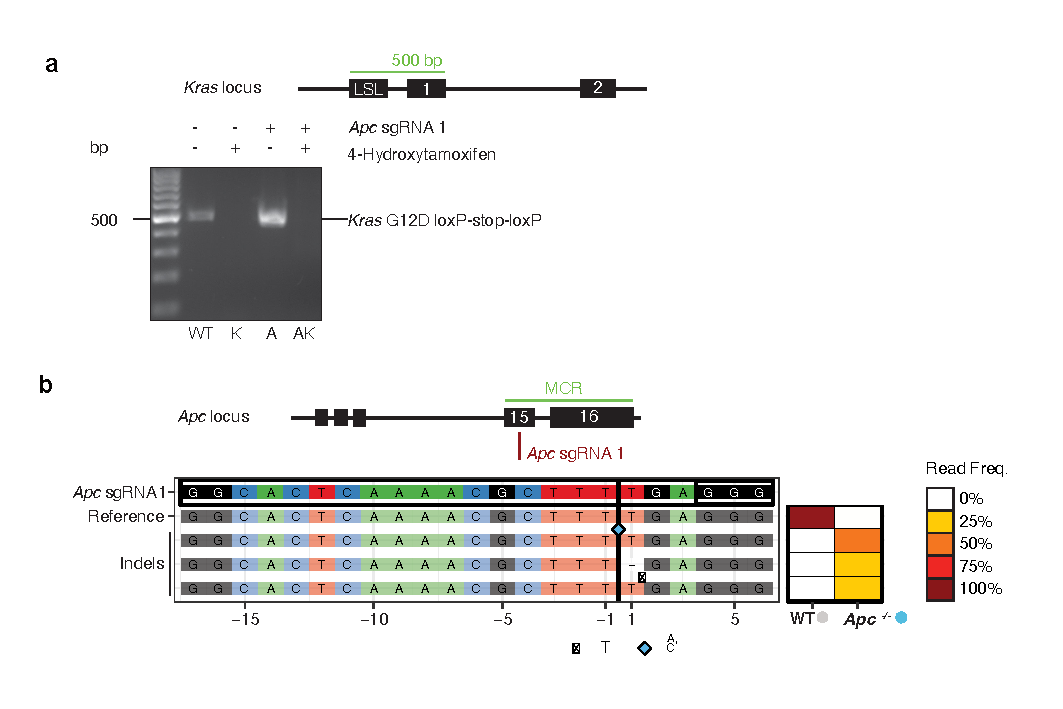
\includegraphics[width=\textwidth,
                height=\textheight,
                keepaspectratio]{figures/adenomaprofiling/pdf/fig_1_1.pdf}
\caption{\textbf{Structural validation of organoid colon adenoma models, a} Allele-specific PCR products of colon organoid models isolated from a transgenic mouse with a conditional tamoxifen inducible KrasG12D/+ allele.
\textbf{b} Amplicon sequencing result of the murine mutation cluster region ortholog for organoids transfected with an Apc targeting sgRNA and Cas9 carrying plasmid. The sequencing results show the presence of 3 different insertion/deletions within the pool of sgRNA treated organoid models. Wildtype sequences are absend within the CRISPR targeted pool, while mutant sequences are absent in the untreated organoid pool.}
\label{fig_a11}
\end{figure}
\bigbreak

Similar to genetically modified human colon organoids (Drost et al., 2015a; Matano et al., 2015), adenoma models showed characteristic niche requirements. Both Apc mutant organoid lines grew independent of the Wnt-signaling activating factors Wnt 3a and R-Spondin1 (Figure \ref{fig_a10}b). In fact, Apc mutant lines showed an increased growth in a Wnt3a and R-Spondin1 free environment when compared to the complete medium. 
Organoid models with an activated KrasG12D allele were less sensitive to removal of EGF from the media. However, as observed before (Drost et al., 2015a), the mutant KrasG12D allele was insufficient to compensate completely for the loss of EGF from the medium. Nevertheless, KrasG12D mutant organoid lines were more resistant to pharmacological inhibition of Egfr signaling (Figure \ref{fig_a10}c). In conclusion, organoid model genotypes were reflected in characteristic growth factor dependencies.


Next, I investigated the effects of mutations in Apc and Kras on both canonical Wnt- and Erk dependent signaling. While the presence of the KrasG12D/+ allele led to an increase in Erk-phosphorylation across models, Apc-/- / KrasG12D/+ organoids showed no marked additional increase in Erk-phosphorylation when compared to KrasG12D/+ organoids (Figure \ref{fig_a10}d). Moreover, Apc-/- / KrasG12D/+ adenoma models showed no significant differences in expression of the Wnt target genes Axin2 and Ccnd when compared to Apc-/- single-mutant models (A) (p > 0.34 for all conditions, Wilcoxon rank sum test) (Figure \ref{fig_a10}e). These results indicate that organoid adenoma models show genotype-dependent activity of characteristic signaling pathways, while there is no extensive crosstalk between the Apc-/-  and KrasG12D/+ allele in mouse colon organoids that that is directly reflected in canonical Wnt- and Erk dependent signaling.  

\bigbreak
\section{Biochemical profiling of organoid models}

To explore comprehensive molecular differences between organoid models, I next performed transcriptome, proteome and lipidome profiling of all four organoid models (Figure \ref{fig_160}). Transcriptome profiling of organoid models showed an increased expression of the stem-cell marker Lgr5 and Wnt-signaling regulators such as Nkd1, Notum, Wif1 and Znrf3 in Apc mutant organoid lines (Figure \ref{fig_160}b). To the contrary, Apc wildtype organoid lines showed an increased expression of epithelial differentiation markers, such as Krt20, Alpp and Abcb1 (P-glycoprotein). Overall, the number of genes with significant expression changes after Apc loss was 2.5 times greater compared to isolated KrasG12D activation (FDR = 0.1, Apc-/-: 44.5\%, KrasG12D/+: 18.3\% of assessed genes). 

\begin{figure}[h]
\centering
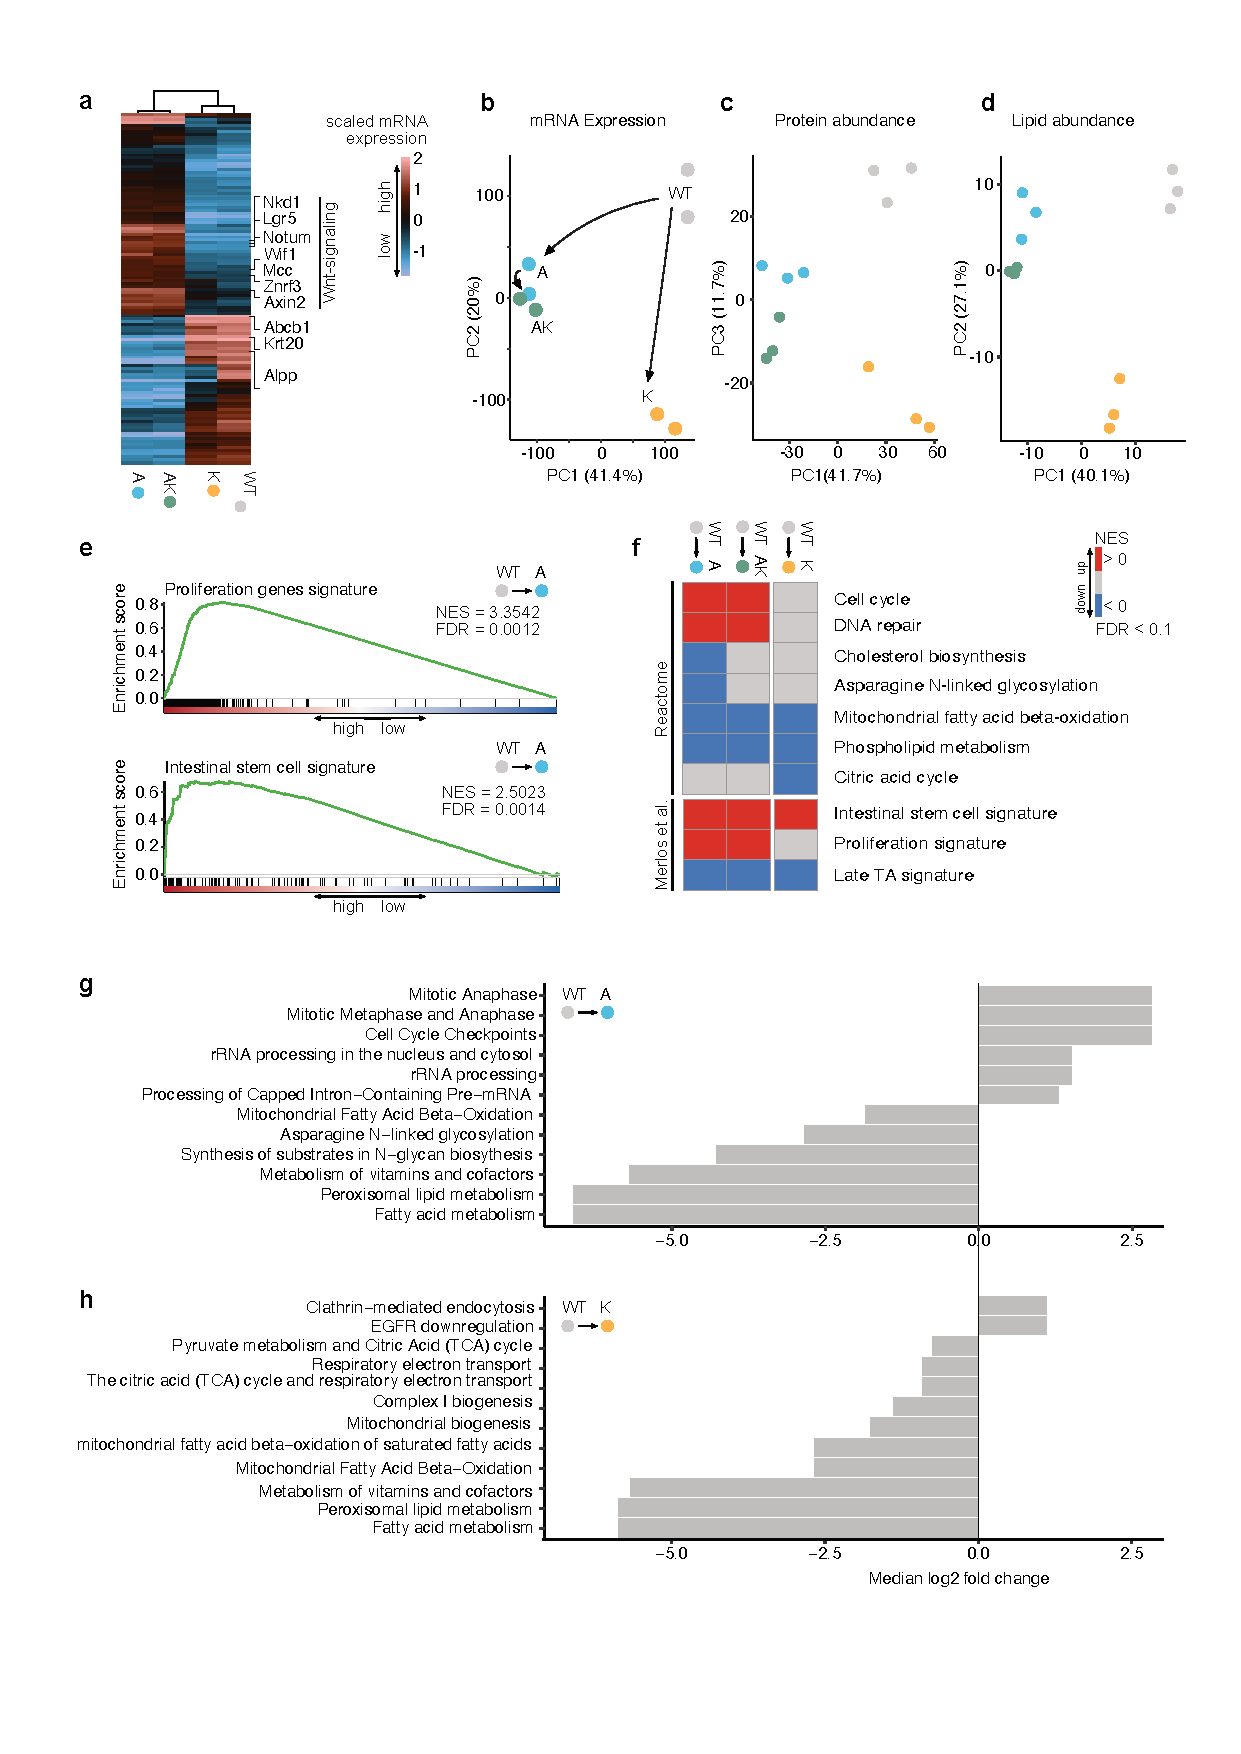
\includegraphics[width=\textwidth,
                height=\textheight,
                keepaspectratio]{figures/adenomaprofiling/pdf/fig_1_6.pdf}
\caption{\textbf{Molecular profiling of organoid adenoma models. a} Differential gene expression of adenoma models. Shown are scaled expression values for the top 125 differentially expressed genes for every organoid line. Selected genes are highlighted. All organoids were cultured for 3 days in WENRAS before exposure to ENR for 4 days. Cell number was controlled between experiments. Whole organoid lysates were analyzed. 
\textbf{b} Transcript abundance data. Shown are the first two principal components of scaled gene expression data. The proportion of variance of each principal component is listed in parenthesis. 
\textbf{c} Protein abundance data. Shown are the first and third principal component of scaled protein expression data. The proportion of variance of each principal component is listed in parenthesis. 
\textbf{d} Lipid species abundance data. Shown are the first two principal components of scaled lipid abundance data. The proportion of variance of each principal component is listed in parenthesis. 
\textbf{e} Loss of Apc leads to increased expression of proliferation and intestinal stem cell associated genes. Shown is a gene set enrichment analysis of differentially expressed genes between Apc mutant and WT organoids. Intestinal gene expression signatures were used according to Merlos et al. NES, normalized enrichment score. 
\textbf{f} Overview of cellular processes in organoid adenoma models. Shown are selected enriched differential gene expression signatures from reactome and Merlos et al. NES, normalized enrichment score. NES > 0 suggests an enriched/ activated biological process. FDR < 0.1. 
\textbf{g} Representative up and down-regulated transcriptional processes after loss of Apc. Expression signatures were sourced from reactome and average log2 fold changes for included transcripts are illustrated. FDR < 0.1.
\textbf{h} Representative up and down-regulated transcriptional processes after activation of oncogenic Kras G12D. Expression signatures were sourced from reactome and average log2 fold changes for included transcripts are shown. FDR < 0.1.}
\label{fig_160}
\end{figure}
\bigbreak


A related observation was made during the analysis of protein abundance. Proteome profiling and imputation identified 3906 gene products in all measured organoid lines. Again, Wnt signaling regulators (Axin2, Notum) were enriched in Apc mutant organoid lines and the number of significantly regulated proteins after Apc loss was 2.5 times greater compared to an isolated KrasG12D activation (FDR = 0.1, Apc-/-: 260, KrasG12D/+: 105 assessed proteins). 

Principal component analysis of both transcriptome, proteome and lipidome data showed a related organization of variance across measurements. Across modalities, the first principal component captured differences between Apc wildtype and Apc mutant organoid models, while the second (in case of proteomics measurements the third) principal component captured differences between wildtype and KrasG12D/+ single-mutant models (Figure \ref{fig_160}b, \ref{fig_160}c and \ref{fig_160}d). In every modality, a high degree of similarity was observed among Apc-/- and Apc-/- / KrasG12D/+ organoid lines. While activation of oncogenic KrasG12D in wildtype organoids led to global changes in transcript, protein and lipid expression, these changes were not as pronounced in organoids without functional Apc. In fact, only the mRNA expression of 91 genes was significantly altered between Apc-/- and Apc-/- / KrasG12D/+ organoids (FDR = 0.1). 

To explore activated biological processes, gene set enrichment analysis on organoid mRNA expression data was performed. The strongest changes in gene expression after loss of Apc were linked to an increased proliferative activity (Figure \ref{fig_160}e). Gene set enrichment analysis of published intestinal cell-proliferation and stem cell signatures showed an enrichment of both signatures in Apc-/- organoids (Figure \ref{fig_160}e) (Merlos-Suárez et al., 2011). In contrast, a signature for differentiating transit-amplifying cells was depleted. Gene set enrichment analysis of Apc-/- / KrasG12D/+ double-mutant organoids showed the same results. 

Next to these published signatures, I explored the enrichment of curated gene sets from the Reactome database (Fabregat et al., 2018). Here, both Apc-/- and Apc-/- / KrasG12D/+ double-mutant lines showed a positive enrichment of cell cycle and DNA repair related genes when compared to wildtype organoids (Figure \ref{fig_160}f and g). Unique to the KrasG12D/+ organoid line was a decreased expression of citric acid cycle and respiratory chain related genes (Figure \ref{fig_160}f and h). This effect, was not observed in Apc-/- / KrasG12D/+ double mutant organoids (Figure 2\ref{fig_160}f). In addition, organoid models with an KrasG12D/+ genotype showed a downregulation of the EGFR receptor, in line with a potential negative feedback response to hyperactivated RAS-MAPK signaling (Figure \ref{fig_160}h). Both Apc-/- and KrasG12D/+ organoid models showed a strong reduction of lipid metabolism and beta-oxidation (Figure \ref{fig_160}f, g, h).

In summary, loss of Apc leads to a global shift in transcript, protein, and lipid abundance in colon organoids, including a strong increase in cell proliferation associated genes. Activation of isolated oncogenic KrasG12D leads to pronounced reduction in citric acid cycle related gene expression while this phenotype was not seen in organoid models with a loss of Apc.

\begin{figure}[h]
\centering
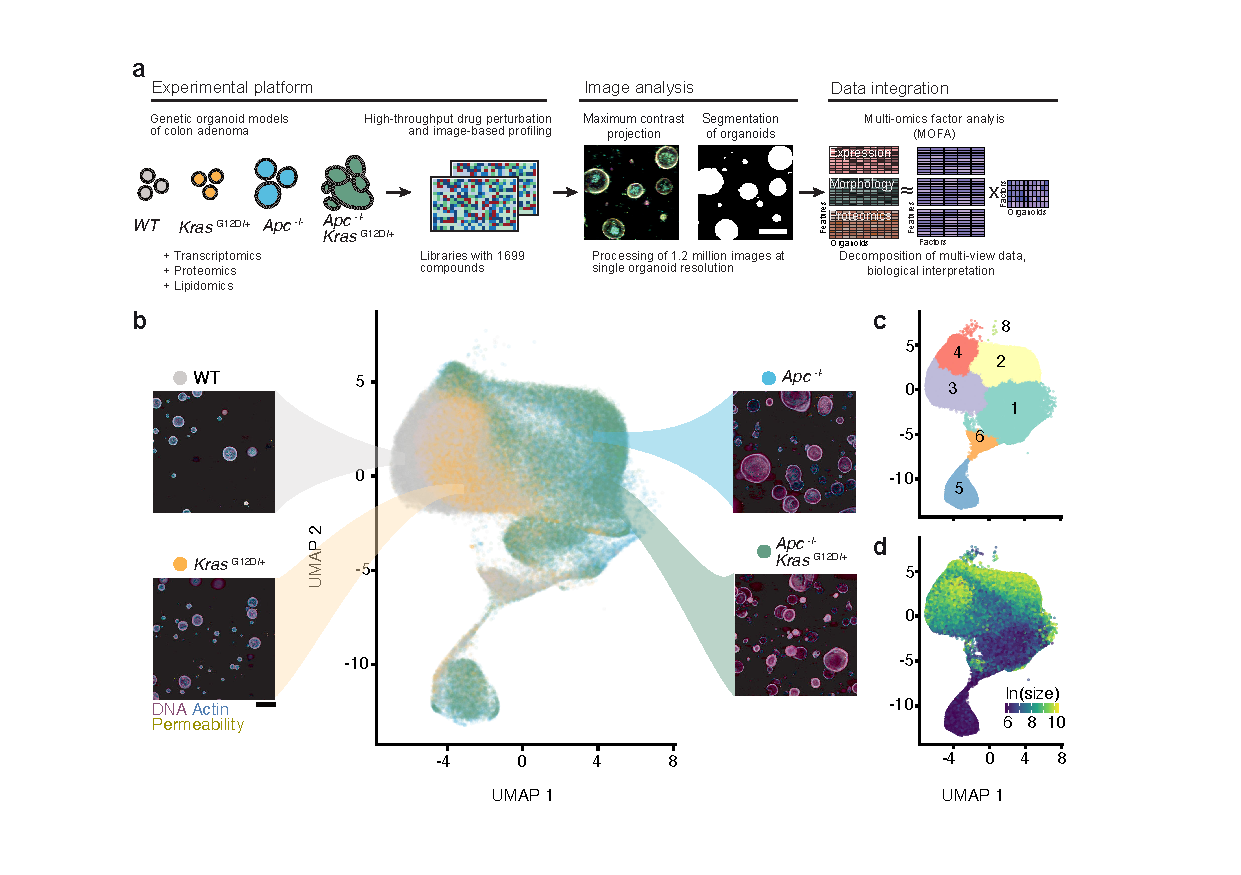
\includegraphics[width=\textwidth,
                height=\textheight,
                keepaspectratio]{figures/adenomaprofiling/pdf/fig_1_2.pdf}
\caption{\textbf{Image-based profiling of organoid adenoma models. a} Overview of experiments. Organoids were isolated from a transgenic mouse model and genetically edited. Organoids were dissociated and evenly seeded in 384-well plates before perturbation with an experimental small molecule library. After treatment, high-throughput fluorescence microscopy was used to capture the morphology of organoids in 16 selected z-layers and 3 channels. 3D imaging data were projected on a 2D plane using a maximum contrast projection. Here, only pixel areas with the largest contrast among the z-axis were retained. Morphological features were computed based on the projection. Untreated organoid morphology, organoid size and drug activity scores were integrated with transcript expression, protein abundance, lipid abundance and genogtype data in a Multi-Omics Factor Analysis (MOFA) model. Figure created with support from Johannes Betge (graphical presentation). 
\textbf{b} Uniform Manifold Approximation and Projection (UMAP) of organoid-level features for a random 5\% sample out of imaged organoids. The identical sample is used for visualizations throughout the figure. Organoid genotype is colorcoded and representative images are displayed (magenta = DNA, cyan = actin, cell permeability = yellow, scale-bar: 200µm). \textbf{c} Graph-based clustering of organoids by morphology with 8 resulting clusters. \textbf{d} Organoid size distribution. Color corresponds to the log-scaled organoid area (dark blue: minimum size, yellow: maximum size).}
\label{fig_120}
\end{figure}
\bigbreak

\newpage
\section{Image-based profiling of organoid models}

To measure how organoids change their biological state as a response to small molecule perturbation, I used the previously developed image-based profiling method to observe organoid morphology. Organoid models of four different genotypes were perturbed with a library of ca. 1700 compounds and morphological profiles were computed (Figure \ref{fig_120}a). A UMAP projection of 25 principal components representing single-organoid morphology showed distinct genotype-dependent morphological states for viable organoids (Figure \ref{fig_120}b). Graph based clustering of organoid morphology profiles resulted in 8 different clusters (Figure \ref{fig_120}c). While developed organoids within cluster 4 and 3 were enriched for Apc+/+ organoid models, cluster 2 and 1 were populated by Apc-/- models. Analogous to gene expression, lipidomics and proteomics representation space, Apc mutant organoid models were less distinct from each other than organoids with a WT and isolated KrasG12D/+ genotype (Figure \ref{fig_140}b). While developed organoids that present with a larger organoid area showed distinct genotype-specific morphologies, small and dead organoids clustered together across genotypes within cluster 5 (Figure \ref{fig_120}c and d). 

\begin{figure}[h]
\centering
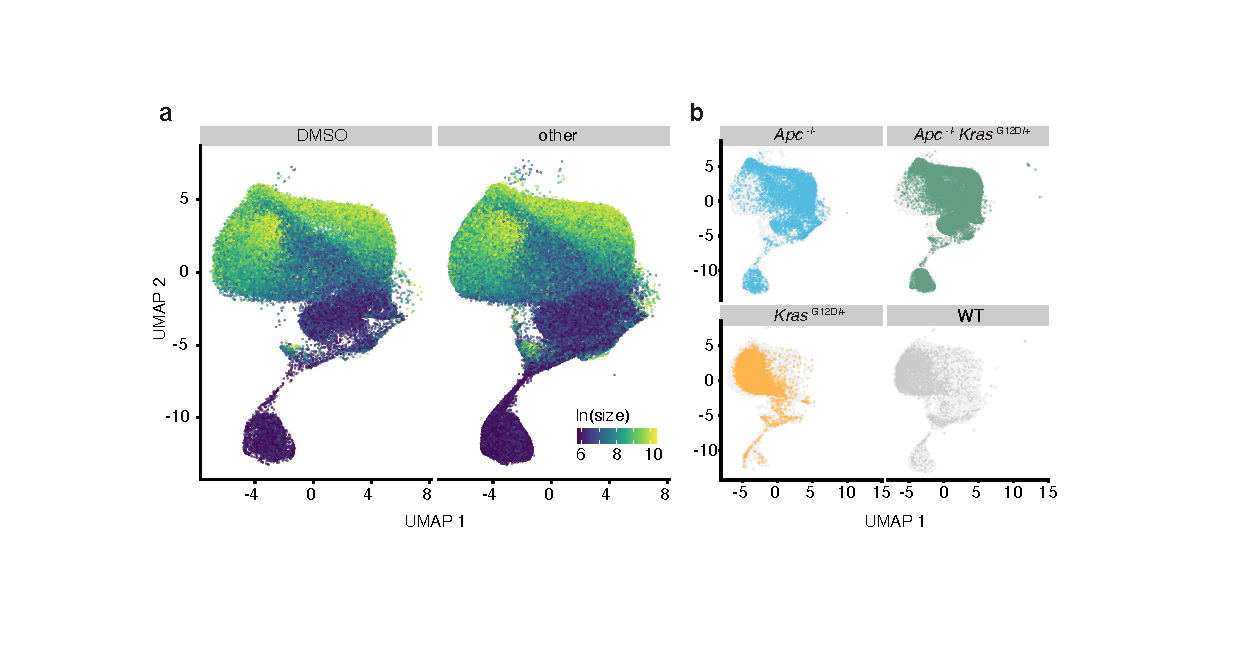
\includegraphics[width=\textwidth,
                height=\textheight,
                keepaspectratio]{figures/adenomaprofiling/pdf/fig_1_4.pdf}
\caption{\textbf{Treatment and genotype dependent effects on organoid morphology distribution. a} UMAP representation of DMSO treated (vehicle) and small molecule treated organoids. \textbf{b}, UMAP embeddings of four organoid genotypes (baseline state = 0.1\% DMSO control-treated organoids), grey background consists of randomly sampled organoids.}
\label{fig_140}
\end{figure}
\bigbreak

The distribution of DMSO-treated organoids and small molecule perturbed organoids in morphological space overlapped strongly (Figure \ref{fig_140}a), possibly because of large amount of treatments that did not alter organoid morphology.

\begin{figure}[h]
\centering
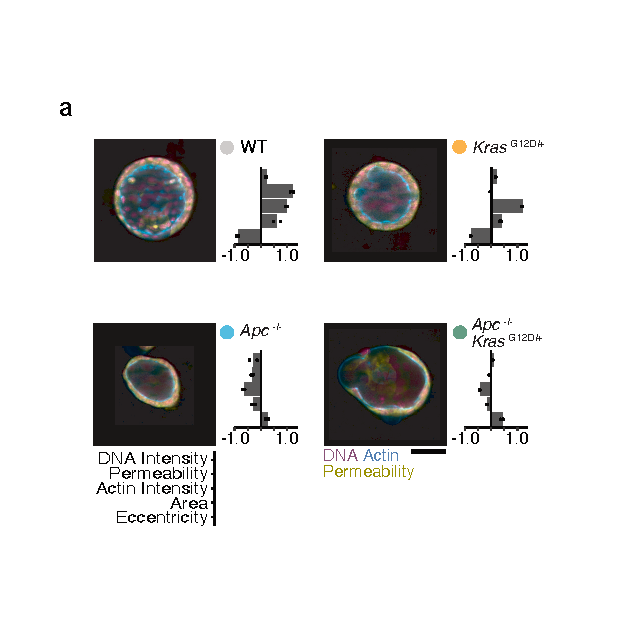
\includegraphics[width=200,
                height=\textheight,
                keepaspectratio]{figures/adenomaprofiling/pdf/fig_1_3.pdf}
\caption{\textbf{Genotype dependent effects on organoid morphology. a} Unperturbed organoid profiles from adenoma models were aggregated. Shown are representative individual organoids with selected features. Points show the mean phenotype for each independent biological replicate. Selected features and their z-scores relative to all single organoid profiles are shown (magenta = DNA, cyan = actin, cell permeability = yellow, scale-bar: 25µm)}
\label{fig_130}
\end{figure}
\bigbreak

When comparing the morphologies of different organoid models in detail, characteristic differences were identifiable (Figure \ref{fig_130}a). DMSO-treated Apc+/+ organoids showed a strong, regular apical actin cytoskeleton (high average actin intensity) that organized the multicellular formation into a regular-patterned spherical morphology (low average eccentricity). In contrast, Apc-/- organoids showed a relative lack of a regular actin cytoskeleton (low average actin intensity) and a irregular, non-spherical morphology (high average eccentricity). 

In summary, developed organoids showed genotype-dependent differences in morphology. Analogous to differences in biochemical state, a primary source of variation was the loss of the tumor suppressor gene Apc. Organoids with truncated Apc presented with a loss of the spherical, potentially structure-conferring, and cell-spanning apical actin cytoskeleton that was observed in Apc +/+ organoid models.

\section{Quantifying small molecule induced phenotypes across organoid models}

\begin{figure}[h]
\centering
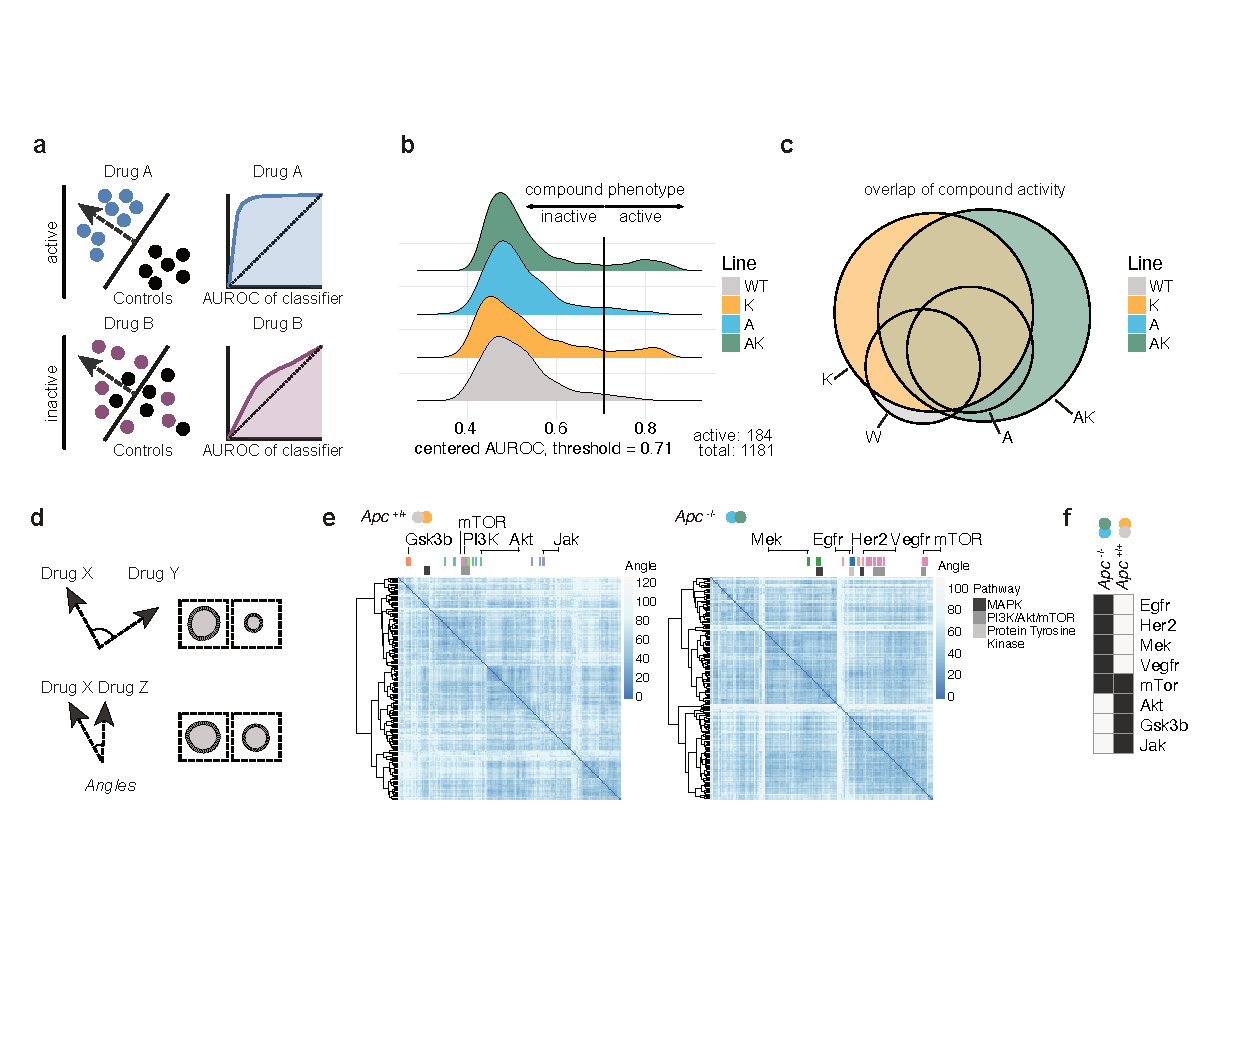
\includegraphics[width=\textwidth,
                height=\textheight,
                keepaspectratio]{figures/adenomaprofiling/pdf/fig_1_5.pdf}
\caption{\textbf{Small molecule activity scoring. a} A logistic regression classifier is trained to distinguish morphology profiles of individual treated and untreated organoids across all available replicates. Afterwards, the classifier is applied to a validation set of organoids and the classification performance is estimated using the area under the receiver operating characteristic curve (AUROC) metric. Method implemented by Jan Sauer.
\textbf{b} Distribution of AUROC compound activity scores for all organoid lines, replicates and perturbations. AUROC scores were centered around 0.5 and treatments for this particular analysis were termed active when classification accuracy exceeded three times the Median Absolute Deviation (MAD) of the AUROC score distribution, an arbitrary threshold. A set of 184 compounds (16\% of all screened small molecules) met the activity criteria. 
\textbf{c} Overlap of active compound treatments across organoid models. Shown is a Euler diagram of active compounds for each line. K (Kras G12D), AK (Apc loss and Kras G12D) and WT are color coded. Plot diagnostics: diagError: 0.011, stress: 0.002.
\textbf{d} Identifying related treatment induced phenotypes. Normal vectors of treatment specific classifiers were compared by calculating the angular distance (related to cosine similarity, ranging from 0-180 degrees). Small angular distance between vectors correspond to a high similarity between the treatment-induced organoid phenotypes. Method implemented by Jan Sauer.
\textbf{e} A map of compound induced phenotypes for Apc mutant and Apc wildtype organoids. Highlighted are clusters of compound induced phenotypes with related targets. Normal vectors for Apc mutant and Apc wildtype organoids were concatenated before angular distance calculation. Method implemented by Jan Sauer.
\textbf{f} Treatment induced phenotypes by organoid genotype. Shown are significantly enriched treatment induced phenotypes for Apc mutant and wildtype organoid models. Clusters of similar phenotypes were tested for overrepresentation of known molecular targets using Fisher’s exact test. Significantly enriched targets are shown. Method implemented by Jan Sauer.
}
\label{fig_150}
\end{figure}
\bigbreak

To study the effect that small molecule perturbations had on organoid models, the classification based approach developed during the study of human cancer organoid phenotypes was used. Briefly, for every treatment and genotype, a linear classifier was trained to distinguish DMSO-treated organoids from treated organoids. The classification performance, expressed as the AUROC obtained on a hold-out dataset, was used to determine the activity of a compound. A high AUROC (approaching 1) is observed for compounds that lead to a treatment-induced organoid morphology that is very distinct from DMSO treated organoids. In contrast a low AUROC (minimum of 0.5) is observed for compounds where the classification performance approaches random guessing (Figure \ref{fig_150}a).

Related to the approach chosen in the previous chapter, active treatments were identified based on the AUROC score that a classifier reached. Given differences in the distribution of AUROC scores between lines, with KRAS G12D/+ organoid lines being shifted towards higher AUROC values, I centered the distribution of AUROC scores around 0.5 and defined an arbitrary activity threshold at 3 times the Median Adjusted Deviation for all tested models (Figure \ref{fig_150}b). A primary source of variation in the genotype-dependent identity of active compounds (16\% of all tested small molecules) was the functional state of Apc, as most active compounds were shared among Apc+/+ and Apc-/- models, while little relative overlap existed between these two alleles (Figure \ref{fig_150}c). As described above, the higher classification performance seen in organoids with the Kras G12D/+ allele, led to a larger number of active drugs identified for these models. A possible reason for this systematic difference in the number of active treatments might be a larger number of developed organoids seen in the images of these models. This difference might be linked to the previously described increased colony-forming capacity seen in Kras G12D/+ colon cancer models.
%% cite paper here

Given the observation that the primary source of variation for drug activity, similar to other biochemical assays, was the state of the Apc allele, I focused the analysis of treatment-induced organoid phenotypes along this axes. Similar to the approach taken in the previous chapter, normal vectors of the logistic regression classifiers were compared by estimating the enclosed angle (Figure \ref{fig_150}d). Normal vectors for organoids with the same Apc allele were concatenated. The resulting clustering of normal vectors by their similarity showed an enrichment for small molecules with related mechanism of action (Figure \ref{fig_150}e and f). For example, EGFR inhibitors were significantly enriched in Apc-mutant organoid lines, while GSK3B-inhibitors, which lead to a stimulation of canonical Wnt signaling, were enriched in Apc-wildtype organoid models, only. 

\section{Multi-omics factor analysis identifies shared factors linking functional and structural biological views}

\begin{figure}[h]
\centering
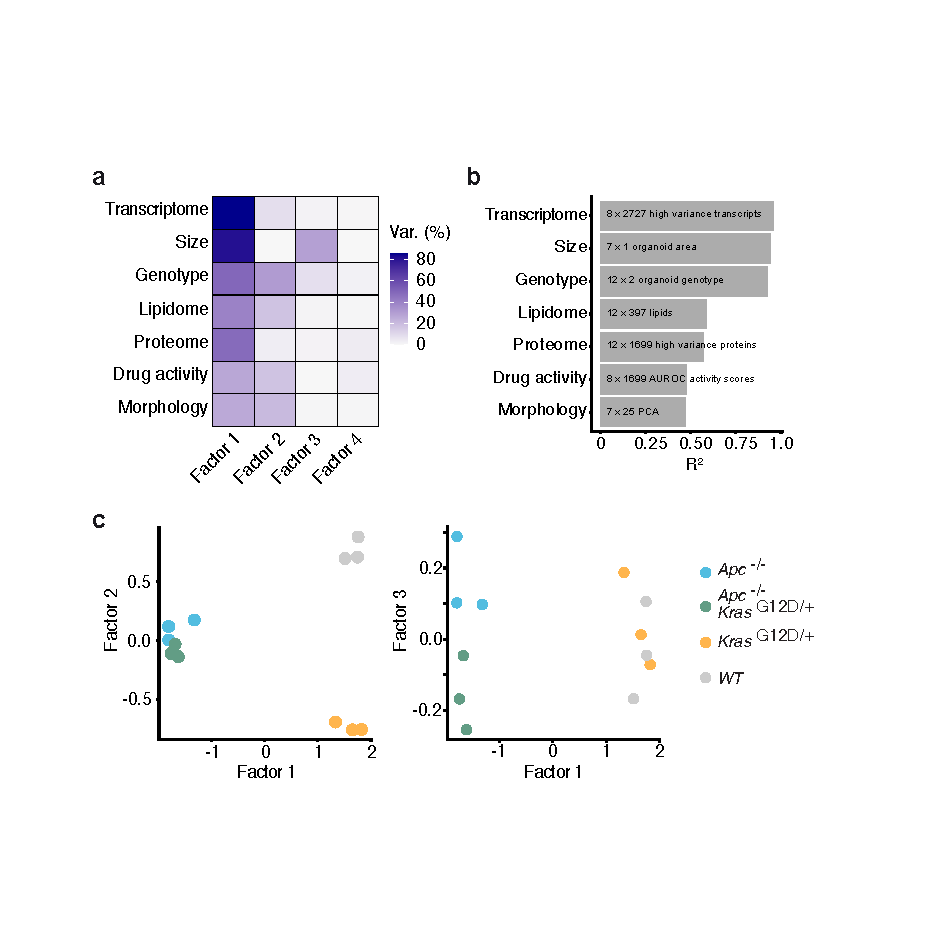
\includegraphics[width=350,
                height=\textheight,
                keepaspectratio]{figures/adenomaprofiling/pdf/fig_1_7.pdf}
\caption{\textbf{Multi-omics factor analysis to identify shared factors linking morphology, size, gene expression, lipidomics, proteomics, genotype and drug activity. a} Percent variance explained by the MOFA model for each factor. Untreated organoid morphology, organoid size and drug activity scores were integrated with genotype, proteomics, lipidomics and mRNA expression data. \textbf{b} Cumulative proportion of total variance explained by each experimental data modality within the MOFA model. \textbf{c}, Visualization of samples in factor space showing factors 1 and 2 as well as factor 1 and 3. Shown are independent replicates for each organoid line. 
}
\label{fig_170}
\end{figure}
\bigbreak

To comprehensively model the biological state of organoid models and explore potential interventions that move organoids in state-space, I performed multi-omics factor analysis (MOFA). Analogous to the process described in chapter 1, feature matrices from different sources were processed and factorized using k=4 factors (Figure \ref{fig_170}a and \ref{fig_180}a). The learned model was based on both functional (e.g. drug activity) and structural (e.g. genotype, proteomics, lipidomics and mRNA expression) information. To reduce the dimensionality of input data, only high variance features from gene expression and proteomics analysis were used.

The resulting factorization explained an overall XX percent of variance across the analyzed views, of which the first three factors captured the majority (XX percent of variance, Figure \ref{fig_170}a). The learned model explained most variance within the mRNA expression and genotype data, while measurements within the organoid morphology data had the lowest explained variance (Figure \ref{fig_170}b). Visual inspection of factors as well as exploration of factor loadings within the genotype view showed that factor 1 explained state differences caused by Apc loss of function, while factor 2 explained state differences caused by the activation of KrasG12D in an Apc+/+ genotype (Figure \ref{fig_170}c and \ref{fig_180}b). In contrast to factor 2, factor 3 captured differences between Kras+/+ and KrasG12D/+ organoids with Apc loss of function, albeit with low overall explained variance. 
% TODO check variance explained

While the initial number of factors is a user-defined feature within MOFA, the method automatically drops excess factors if they are not considered effective based on an applied automatic relevance determination (ARD) prior. Increasing the number of factors above k=4 in this analysis, did not lead to an increased number of interpretable factors. In fact, factor 4 already did not capture differences between organoid genoypes and was not interpretable from a biological point of view (Figure \ref{fig_180}b). This observation and the fact that this study explored the biological effects of two oncogenic genetic events both in isolation and in concert reveals, I speculate, a potential conceptual intersection of representation learning methods, such as MOFA, and the theory of genetic interactions which will be explored in the last chapter of this thesis. 

\begin{figure}[h]
\centering
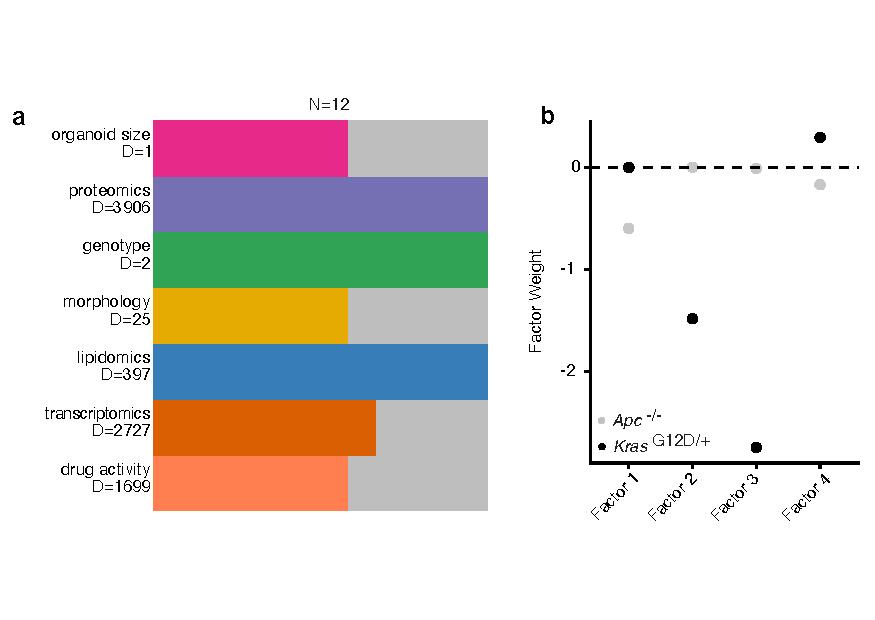
\includegraphics[width=300,
                height=\textheight,
                keepaspectratio]{figures/adenomaprofiling/pdf/fig_1_8.pdf}
\caption{\textbf{Multi-omics factor analysis input data and loadings. a} measurement modalities, dimensionality and number of measurements. A third replicate of measurements were available for proteomics and lipidomics only. \textbf{b} Factor loadings for genotype information.} 
\label{fig_180}
\end{figure}
\bigbreak

\section{A canonical Wnt signaling associated program caused by Apc loss}

To understand the molecular changes associated with factor 1, factor loadings for mRNA expression data were analyzed using Reactome gene-set enrichment analysis (Figure \ref{fig_190}a). Three clusters of biological processes were significantly associated with a negative factor loading, caused by Apc loss-of-function: 1) Mitotic Anaphase related processes, including spindle checkpoints; 2) Mitotic S-phase, including DNA replication and 3) DNA repair mechanisms, including homology directed repair. 

In line with the enrichment of processes seen in cell proliferation, factor 1 loadings were associated with an enrichment of a previously described intestinal proliferation signature (Figure \ref{fig_190}c) and an LGR5+ instestinal stem cell identity signature (Figure \ref{fig_190}b). These findings are in line with the long-standing evidence that loss of Apc leads to a hyperactivation of canonical Wnt signaling, which in turn leads to increased intestinal cell proliferation and Myc-dependent changes towards a stem-like cell state.
%TODO cite Myc paper
%TODO Wnt signaling dependent effects

When focusing on factor loadings of compound activity measurements, a low factor 1 score was significantly linked to increased sensitivity towards small molecules targeting microtubuli and focal adhesion kinase (FAK, Figure \ref{fig_190}d). This morphological sensitivity was presented itself primarily as reduced organoid size and number relative to the DMSO vehicle control (Figure \ref{fig_190}e).

%\begin{figure}[h]
%\centering
%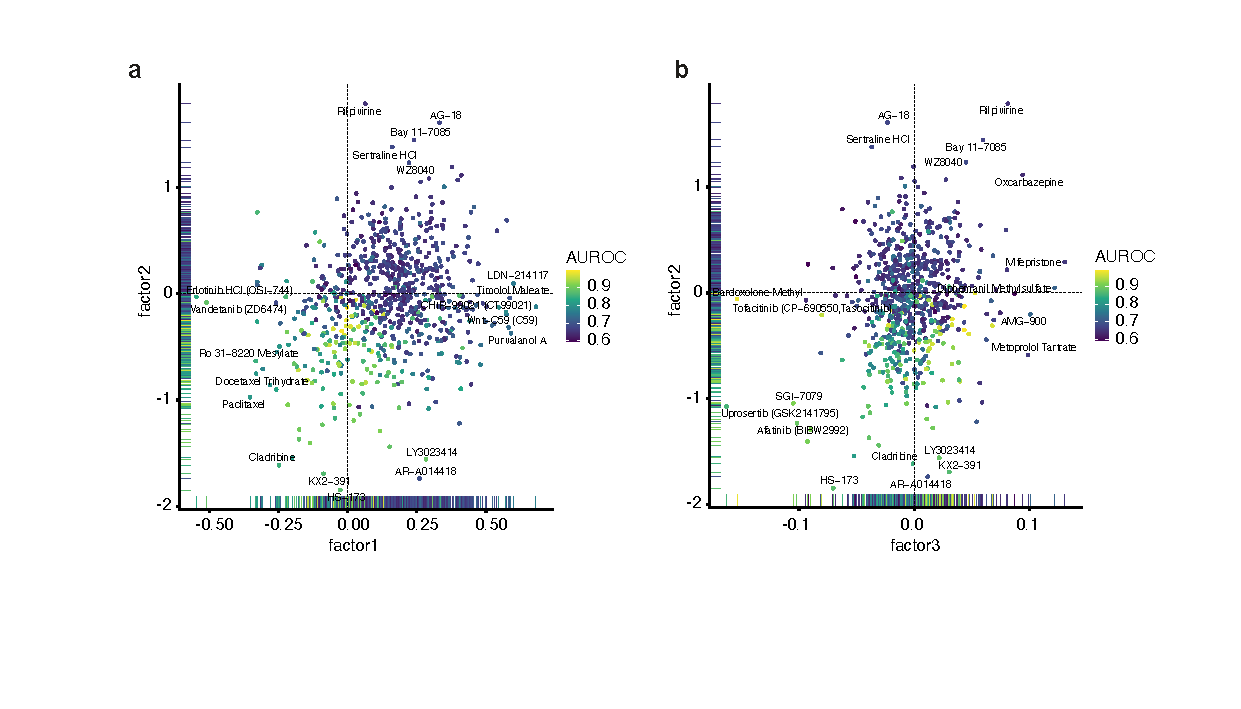
\includegraphics[width=\textwidth,
%                height=\textheight,
%                keepaspectratio]{figures/adenomaprofiling/pdf/fig_1_9.pdf}
%\caption{\textbf{Factor loadings for drug activity. a} Factor 1 and 2 loadings, and \textbf{b} Factor 1 and 3 loadings. Average drug activity score (AUROC) is color coded.}
%\label{fig_180}
%\end{figure}
%\bigbreak

\begin{figure}[h]
\centering
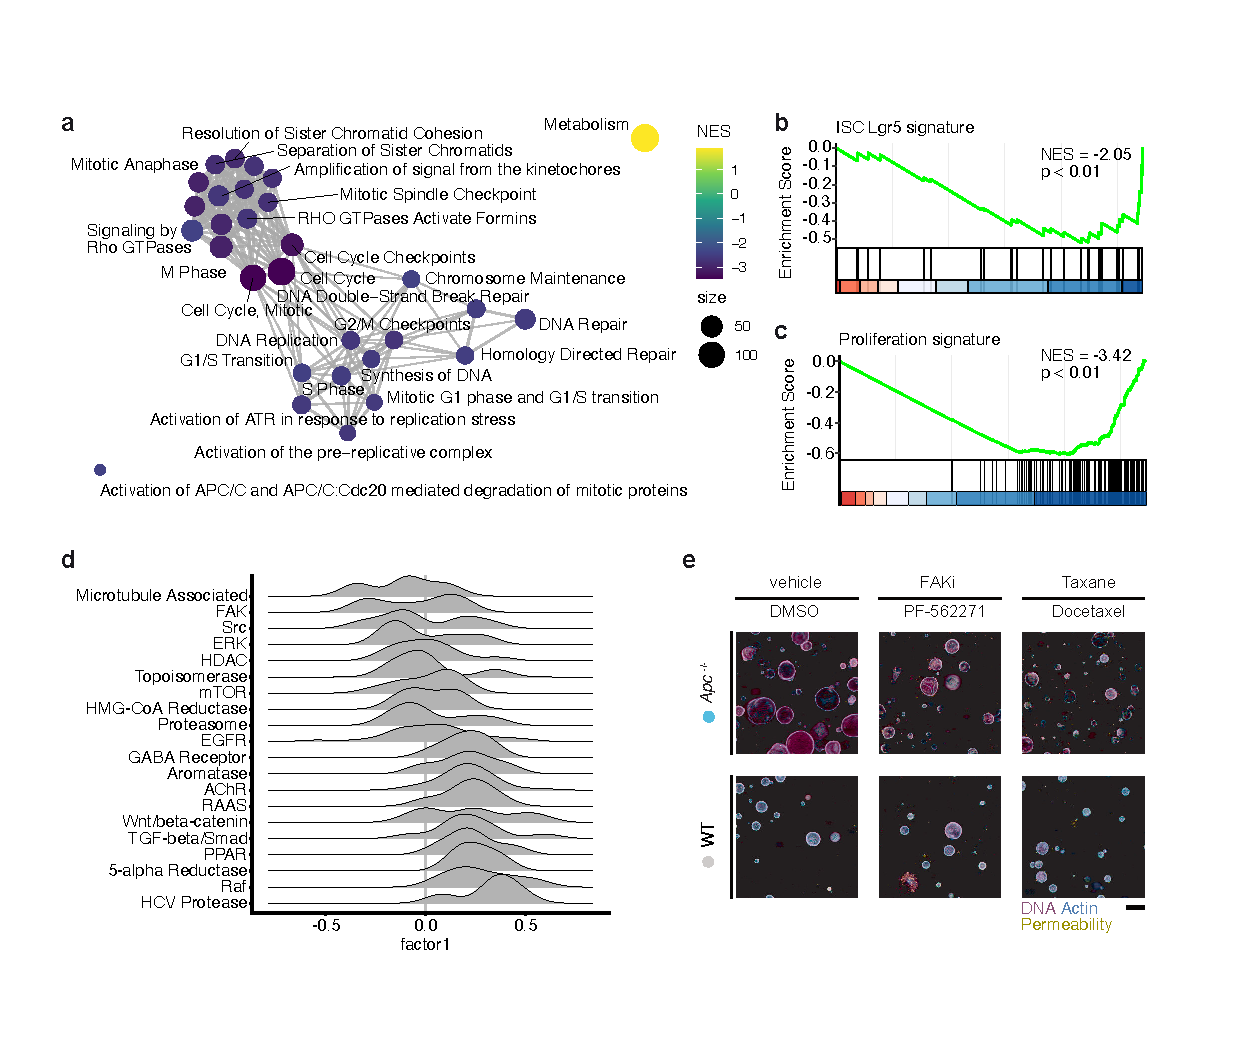
\includegraphics[width=\textwidth,
                height=\textheight,
                keepaspectratio]{figures/adenomaprofiling/pdf/fig_2_1.pdf}
\caption{\textbf{Factor 1, canonical Wnt signaling. a} Gene-set enrichment network of factor 1 gene expression loadings. An edge connects Reactome pathways with more than 20\% overlap. Central enriched processes include mitosis, DNA replication and DNA damage repair. \textbf{b and c} Gene set enrichment results of the "Lgr5 intestinal stem cell" and "proliferation" signature by Merlos-Suarez et al. over ranked factor 1 gene expression loadings (ranking from high factor 1 loading to low factor 1 loading, NES = normalized enrichment score). \textbf{d} Distributions of drug activity loadings grouped by drug target for factor 1. \textbf{e} Example images of compound treated organoids with WT or Apc-/- genotype. Representaধve images are displayed (magenta = DNA, cyan = actin, yellow = cell permeability, scale-bar: 200μm).}
\label{fig_190}
\end{figure}
\bigbreak

In contrast to microtubuli and FAK inhibitors, the average activity scores of small molecules targeting Wnt signaling was associated with increased factor 1 scores (Figure \ref{fig_190}d). Further exploration of the association between the AUROC score and Apc genotype showed that small molecule inhibitors of the canonical Wnt secretion pathway protein Porcupine (Porcn), IWP-L6 and LGK-974, were more active in Apc WT organoids relative to their Apc-/- counterparts (Figure \ref{fig_199}a). In contrast, this effect was not observable for PRI-724, a small molecule inhibitor targeting the interaction of beta-catenin and CREB-binding-protein (\ref{fig_199}a). These differences in drug activity scores among these small molecule inhibitors are most likely related to their different targets' relative location to Apc in the canonical Wnt signaling cascade. While Porcn-dependent Wnt secretion is generally upstream of the destruction complex, the interaction of beta-catenin and CREB-binding-protein is located downstream of it. As a consequence, inhibition of destruction complex function by loss of Apc is expected to render cells less sensitive to perturbations of the Wnt secretion cascade than perturbations of transcription factor binding properties (Figure \ref{fig_199}b). 

Next do factor related differences in morphological compound sensitivity, I analyzed the association of factor 1 weights with lipid species. High concentrations of cholesterol esters were associated with a low factor 1 score (seen in Apc-/- organoids), while elevated concentrations of phosphatidic acid species were linked to a high factor 1 score (figure \ref{fig_199}c).


\begin{figure}[h]
\centering
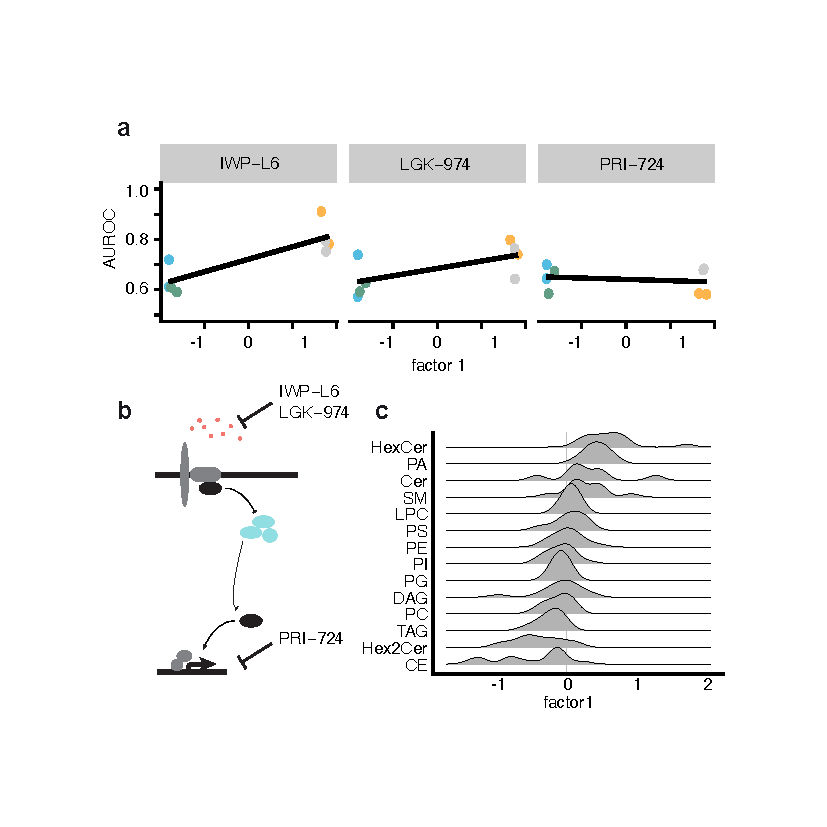
\includegraphics[width=\textwidth,
                height=\textheight,
                keepaspectratio]{figures/adenomaprofiling/pdf/fig_2_2.pdf}
\caption{}
\label{fig_199}
\end{figure}
\bigbreak

\section{An oncogene-induced senescence program caused by isolated KrasG12D activation}
Myc down


\section{mTOR}


\begin{figure}[h]
\centering
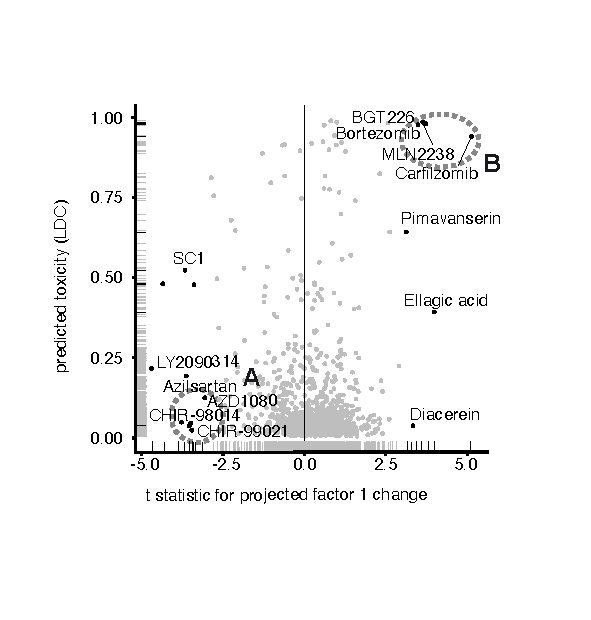
\includegraphics[width=\textwidth,
                height=\textheight,
                keepaspectratio]{figures/adenomaprofiling/pdf/fig_2_3.pdf}
\caption{}
\label{fig_180}
\end{figure}
\bigbreak

\begin{figure}[h]
\centering
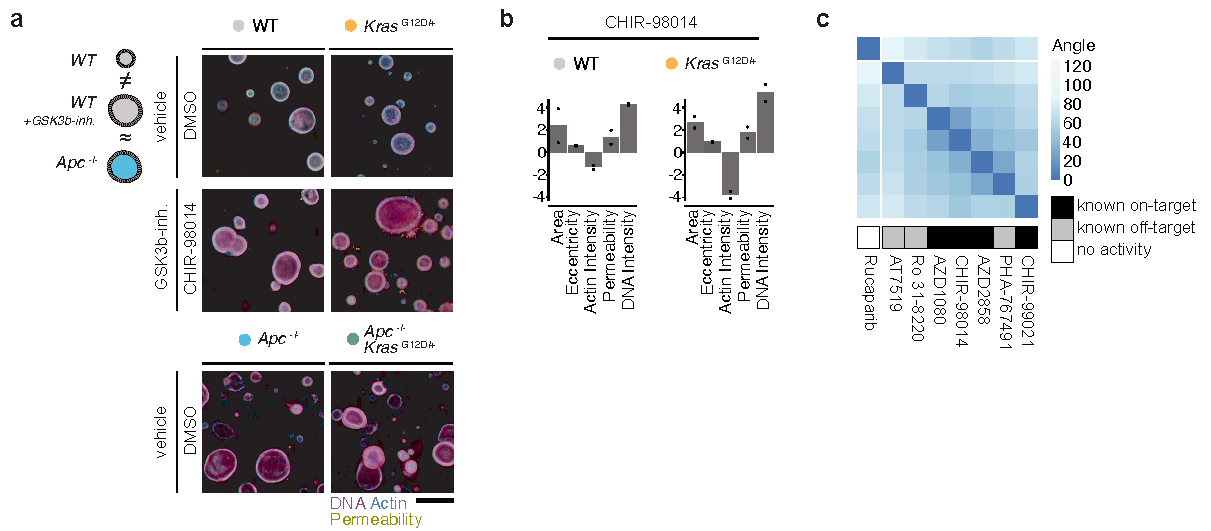
\includegraphics[width=\textwidth,
                height=\textheight,
                keepaspectratio]{figures/adenomaprofiling/pdf/fig_2_4.pdf}
\caption{}
\label{fig_180}
\end{figure}
\bigbreak

\begin{figure}[h]
\centering
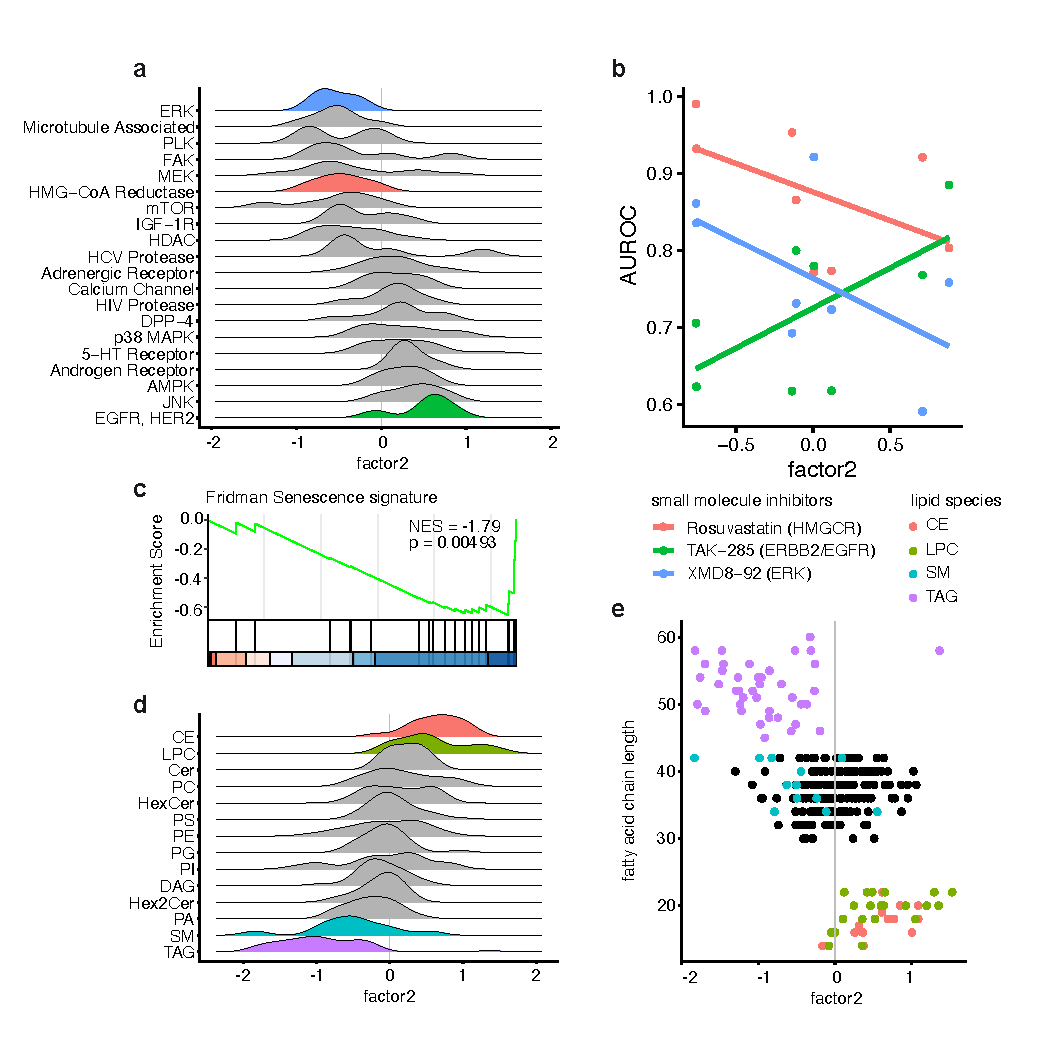
\includegraphics[width=\textwidth,
                height=\textheight,
                keepaspectratio]{figures/adenomaprofiling/pdf/fig_3_1.pdf}
\caption{}
\label{fig_180}
\end{figure}
\bigbreak

\begin{figure}[h]
\centering
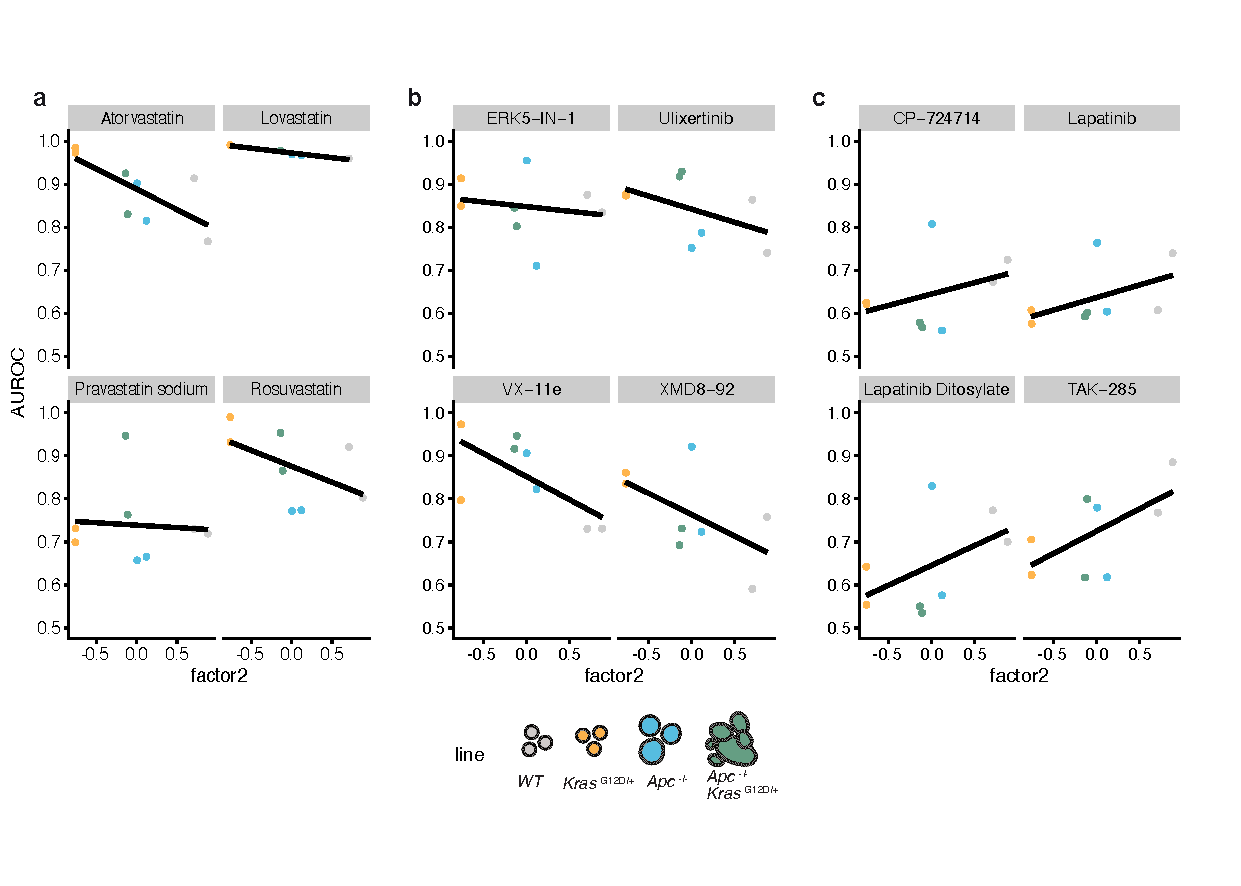
\includegraphics[width=\textwidth,
                height=\textheight,
                keepaspectratio]{figures/adenomaprofiling/pdf/fig_3_2.pdf}
\caption{}
\label{fig_180}
\end{figure}
\bigbreak

\begin{figure}[h]
\centering
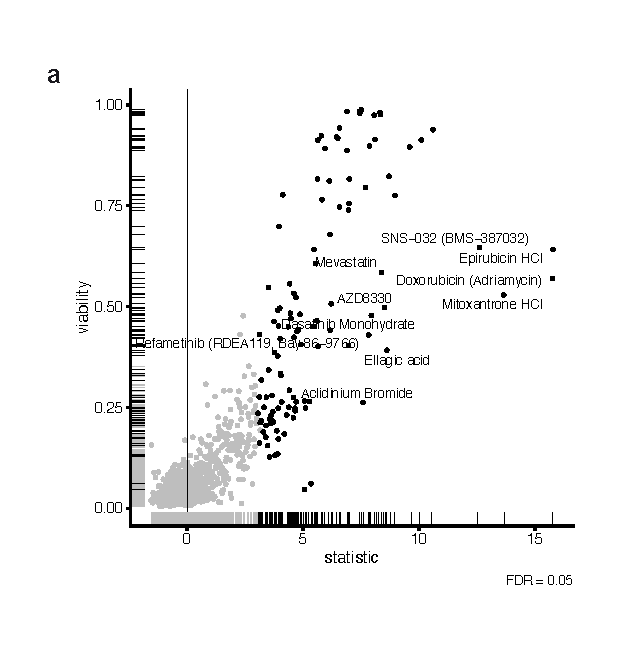
\includegraphics[width=\textwidth,
                height=\textheight,
                keepaspectratio]{figures/adenomaprofiling/pdf/fig_3_3.pdf}
\caption{}
\label{fig_180}
\end{figure}
\bigbreak

\begin{figure}[h]
\centering
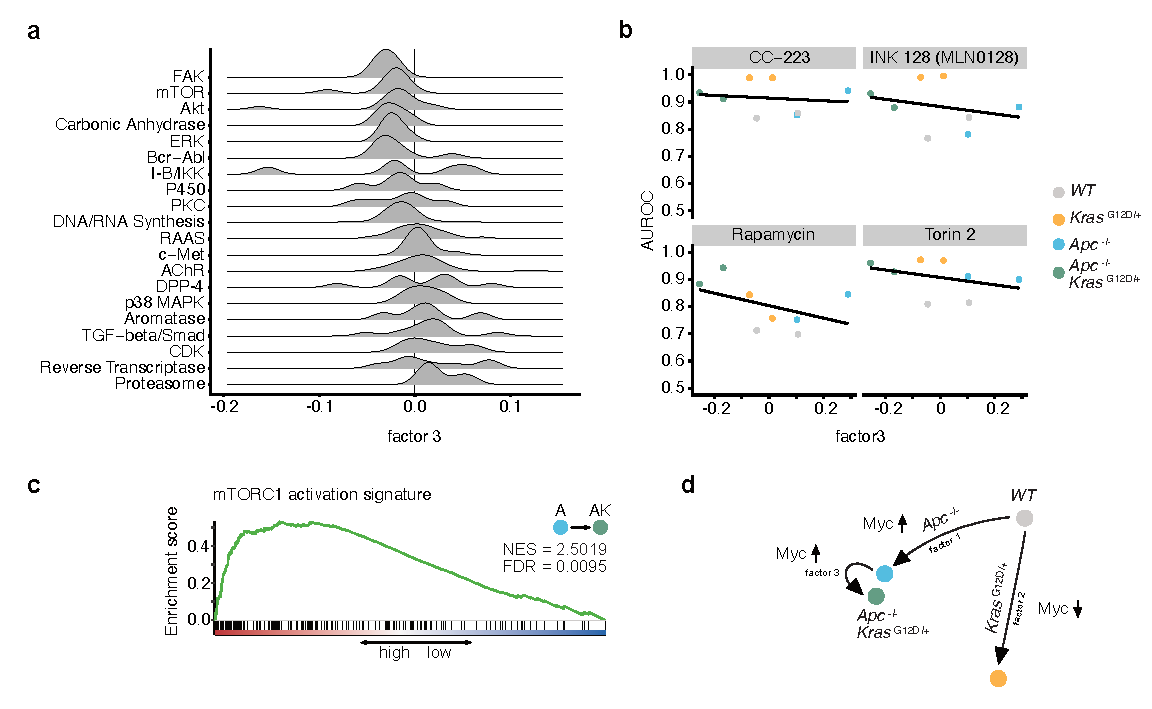
\includegraphics[width=\textwidth,
                height=\textheight,
                keepaspectratio]{figures/adenomaprofiling/pdf/fig_4_1.pdf}
\caption{}
\label{fig_180}
\end{figure}
\bigbreak

\begin{figure}[h]
\centering
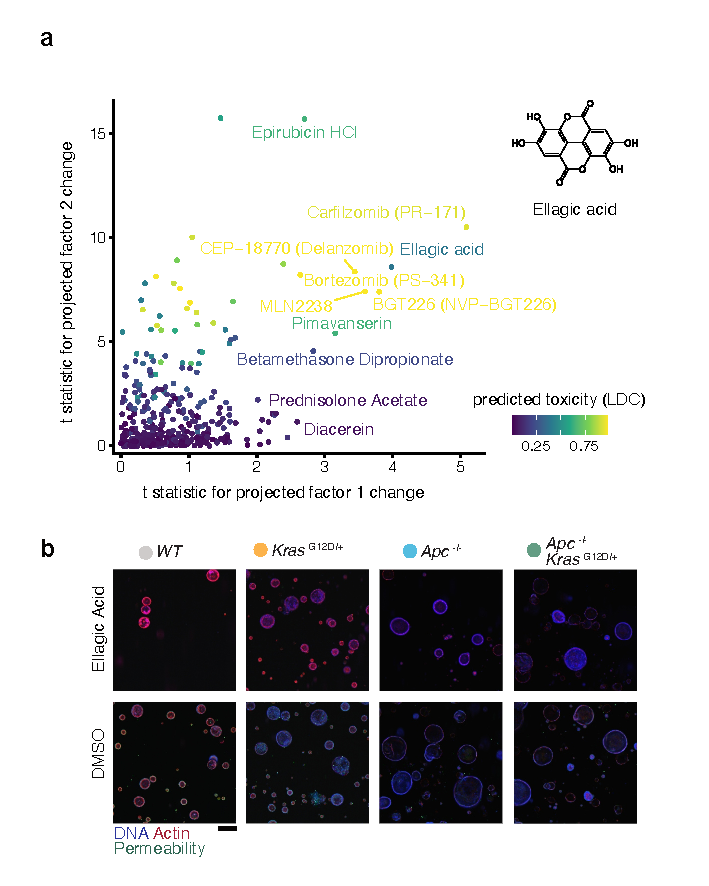
\includegraphics[width=\textwidth,
                height=\textheight,
                keepaspectratio]{figures/adenomaprofiling/pdf/fig_5_1.pdf}
\caption{}
\label{fig_180}
\end{figure}
\bigbreak

\end{flushleft}